\cleardoublepage
\chapter{Koopmans spectral functionals\label{ch:koopmans-theory}}

In this chapter, we describe in detail the theoretical framework of Koopmans functionals, a particular class of orbital-density-dependent functionals that provide the excitation energies of the system -- upon electron addition or removal -- with high level of accuracy. \cref{sec:koopmans-spectral-functionals} is devoted to the concepts of linearization and screening, the two fundamental aspects at the foundation of any Koopmans-compliant functional; we also describe the variational procedure characterizing an orbital-density-dependent approach, which differs substantially from that of typical DFT methods. The connection between Koopmans functionals and many-body perturbation theory is instead discussed in \cref{sec:koopmans-vs-mbpt}. The chapter is closed by a summary of the key concepts, \cref{sec:ch3-summary}.

\clearpage
\section{Koopmans spectral functionals\label{sec:koopmans-spectral-functionals}}
In density-functional theory any observable, including the direct and inverse photoemission spectra, is a functional of the ground-state electronic density. However, often the challenge is to find a way to extract such information once the ground state of the system is determined. Moreover, the existence of an implicit connection does not imply that any observable has an explicit expression in terms of the density, and often we have to rely on different strategies to compute some physical properties. As discussed in \cref{ch:theoretical-background}, computing spectral properties at the DFT level is generally complicated, and even for the first ionization energies we have to resort to GKS schemes or on the $\Delta$SCF method\footnote{The $\Delta$SCF method allows to compute the first ionization energies of the system from total energy differences; it involves calculations on systems at different particle numbers -- $N$, $N-1$, and $N+1$ -- whose ground-state energy differences directly relate to IP and EA.}; the latter, in particular, works only when the densities of the HO and LU orbitals do not delocalize too much, and therefore it inevitably fails in extended systems. Alternatively, we can resort to dynamical approaches -- such as MBPT -- but this normally requires a high computational cost.

Koopmans spectral functionals take place in this framework targeting the electron addition and removal energies, by means of a variational approach. As we shall see, this requires to go beyond the boundaries of KS-DFT and to embody some features of the dynamical self-energy, in order to better describe the quasiparticles. This is achieved via the imposition of a state-dependent condition that shapes Koopmans functionals and makes them dependent on the density of each individual orbital (rather than the total electronic density); effective potentials resulting from such functionals inherit the same orbital-density-dependence (ODD) and closely resemble a simplified version of the frequency-dependent self-energy.

The formalism of Koopmans functionals grounds on the three fundamental concepts: \emph{linearization}, \emph{screening}, and \emph{localization}. The first two aspects will be discussed in \cref{sec:koopmans-condition} and \cref{sec:screening-parameters}, respectively -- and underlie the construction of any Koopmans functional; the concept of \emph{localization} is related to the nature of the orbital densities minimizing the functional, and it is described in detail in \cref{ch:koopmans-periodic}. In \cref{sec:koopmans-functionals}, we define Koopmans functionals, while \cref{sec:variational-procedure} is devoted to the technicalities of the variational procedure which, due to the ODD nature of the functional, is more complex than in a standard KS-DFT framework. Finally, in \cref{sec:koopmans-hamiltonian}, we give a definition of the Koopmans Hamiltonian.

\subsection{Koopmans' condition\label{sec:koopmans-condition}}
In \cref{sec:pwl-energy,sec:deriv-dis}, we discussed the connection between PWL and first ionization energies. For a functional affected by deviation from PWL -- we remark that this could mean that the energy is non-linear at fractional number of electrons and/or the relative position of the energies at integer numbers is not correct -- the left and right energy derivatives do not correspond to the IP and EA of the system. Derivatives require the knowledge of the energy only in an arbitrary small neighborhood around an integer point, thus they allow to compute the first ionization energies (and thereon the band gap) without involving calculations at different particle numbers. Ideally, we would like such energy derivatives to be connected to the eigenvalues of some effective one-particle Hamiltonian, namely
%
\begin{subequations}
    \begin{align}
        E^N - E^{N-1} &= \left. \frac{dE}{dN} \right|_{N-s} = \left. \frac{dE}{df_{\rm HO}} \right|_{s} = \varepsilon_{\rm HO} \label{eq:pwl-frontier-orbitals-ip}\\
        E^{N+1} - E^N &= \left. \frac{dE}{dN} \right|_{N+s} = \left. \frac{dE}{df_{\rm LU}} \right|_{s} = \varepsilon_{\rm LU} \label{eq:pwl-frontier-orbitals-ea},
    \end{align}
    \label{eq:pwl-frontier-orbitals}
\end{subequations}
%
where $f_{\rm HO}$ and $f_{\rm LU}$ are the occupations of the HO and LU orbitals, and we made use of Janak's theorem \eqref{eq:janak-th}; $s$ is any number between 0 and 1, and allows to include the property of PWL: $\varepsilon_{\rm HO}$ and $\varepsilon_{\rm LU}$ are indeed independent from $s$, therefore the derivatives appearing in Eqs.~\eqref{eq:pwl-frontier-orbitals} are constant for any value of $s$. KS-DFT fulfills only \cref{eq:pwl-frontier-orbitals-ip}, and only at an exact level, while GKS schemes approximately satisfy also \cref{eq:pwl-frontier-orbitals-ea} \cite{seidl_generalized_1996,cohen_fractional-charge_2008,stein_fundamental_2010}.

Ionization potentials and electron affinities are only the first-order ionization energies, and for a method that aims to deliver all the electron and hole removal energies, Eqs.~\eqref{eq:pwl-frontier-orbitals} are clearly not sufficient. In addition to being an exact property, the PWL facilitates the connection between total energy differences and energy derivatives (and, ultimately, the eigenvalues). The idea then, is to define a similar condition that generalizes Eqs.~\eqref{eq:pwl-frontier-orbitals}, by extending them to all the orbitals in the system, and ultimately dress the eigenvalues with the meaning of quasiparticle energies. This \emph{generalized PWL} \cite{dabo_non-koopmans_2009,dabo_koopmans_2010} condition reads as
%
\begin{equation}
    \frac{dE}{df_i} = \lambda_i = {\rm const} ,
    \label{eq:koopmans-condition}
\end{equation}
%
where $f_i$ is the occupation of the $i$-th orbital. As we shall see in the following section, $\lambda_i$ is the expectation value of the effective (Koopmans) Hamiltonian over the wave function corresponding to the $i$-th orbital, and it is designed to match the energy difference $E^N - E^{N-1}_i$, or $E^{N+1}_i - E^N$, where $E^{N \pm 1}_i$ are the relaxed energies resulting from the removal of an electron or a hole from the $i$-th orbital. \cref{eq:koopmans-condition} nearly resembles Janak's result: in particular, in the basis of the Hamiltonian's eigenvectors, $\lambda_i$ becomes the eigenvalue $\varepsilon_i$ and \cref{eq:koopmans-condition} takes the form of \cref{eq:janak-th}. However, the two results should not be confused, as Janak's theorem does not assume any particular dependence on the occupations for the energy derivatives, whereas the generalized PWL condition imposes that each $\lambda_i$ is independent on $f_i$.

The generalized PWL can also be seen as an extension of Koopmans' theorem. By integrating \cref{eq:koopmans-condition} over $f_i$, between 1 and $s$ (where $s$ can take any value between 0 and 1), we find for the electron removal process
%
\begin{equation}
    E^N - E^{N-1+s}_i = \lambda_i (1-s) .
    \label{eq:generalized-koopmans-th}
\end{equation}
%
When the electron is fully removed ($s=0$), \cref{eq:generalized-koopmans-th} turns into the main result of Koopmans' theorem \eqref{eq:koopmans-theorem-noncanonical}; the same outcome can be obtained for electron addition processes. The generalized PWL condition can then be seen as an extension of Koopmans' theorem to fractional number of particles and, therefore, it is also referred to as \emph{Koopmans' condition}.

\subsection{Koopmans functionals\label{sec:koopmans-functionals}}
Koopmans spectral functionals are designed to satisfy \cref{eq:koopmans-condition}, and for this reason are also called Koopmans-compliant (KC). The idea is to start from some density-functional approximation -- called from now on \emph{base functional}, and generically indicated with $E^{\rm DFT}$ -- and add a KC term which makes the whole expression compliant with the Koopmans' condition. Additionally, we will require that the base functional is not corrected at integer occupations, whereas the KC term should correct the energy only at fractional occupations. Given the state-dependent nature of \cref{eq:koopmans-condition}, the corrective term can be split into different contributions ($\Pi_i$), one for each single-particle state, which brings to the first (coarse) definition of Koopmans functionals  \cite{dabo_non-koopmans_2009,dabo_koopmans_2010}:
%
\begin{equation}
    E^{\rm KC} = E^{\rm DFT} + \sum_i \Pi_i^{\rm} .
    \label{eq:kc-functional-coarse}
\end{equation}
%
By inserting the right-hand side of the expression above into \cref{eq:koopmans-condition}, we obtain
%
\begin{equation}
    \frac{d\Pi_i}{df_i} = - \frac{dE^{\rm DFT}}{df_i} + \lambda_i ,
    \label{eq:pi-term-derivative}
\end{equation}
%
where $\Pi_i$, by construction, depends only on the occupation of the $i$-th orbital -- i.e. $d\Pi_i / df_j = \delta_{ij}$. In this context, the occupation numbers are treated as parameters taking values between 0 and 1, and all the quantities should be defined accordingly: for the total density and the non-interacting kinetic energy we should then consider Janak's expressions, given by Eqs.~\eqref{eq:janak-kinetic} and \eqref{eq:janak-density}. By integrating \cref{eq:pi-term-derivative} between 0 and $s$, we find that the KC term $\Pi_i$ can be expressed as
%
\begin{equation}
    \begin{split}
    \Pi_i(s) &= - \int_0^{s} \frac{dE^{\rm DFT}}{df_i} df_i + \lambda_i s =
    - \int_0^{s} \braket{\phi_i|\hat{h}^{\rm DFT}|\phi_i} df_i + \lambda_i s \\
    &= \{ E^{\rm DFT}(f_i=s) - E^{\rm DFT}(f_i=0) \} + \lambda_i s ,
    \end{split}
    \label{eq:pi-term-general}
\end{equation}
%
where $\hat{h}^{\rm DFT}$ is the effective Hamiltonian resulting from the derivative of the base functional, and in the second equality we used the non-canonical version of Janak's theorem\footnote{It can be showed that Janak's theorem applies also to sets of orbitals other than the eigenvectors, provided that they yield the same ground-state density. In this case, the occupation numbers and the eigenvalues appearing in \cref{eq:janak-th} are replaced by the diagonal elements of the occupation number matrix and of the Hamiltonian, respectively, represented on the set of non-canonical orbitals.}. We also used the fact that the initial hypothesis of zero correction at integer occupations: $\Pi_i(f_i=0) = 0$. Likewise, by using in \cref{eq:pi-term-general} the fact that also for $s=1$ the $\Pi_i$ term should be identically zero, we find that $\lambda_i$ is defined as
%
\begin{equation}
    \lambda_i = \int_0^{1} \frac{dE^{\rm DFT}}{df_i} df_i = E^{\rm DFT}(f_i=1) - E^{\rm DFT}(f_i=0) ,
    \label{eq:lambda-definition}
\end{equation}
%
which sets the energy derivatives to be equal to a difference of total energies calculated at the level of the chosen base functional. The two latter equations provide the definition for the Koopmans corrective terms, which leave the energy of the base functional unchanged at integer occupations, and linearize it at fractional occupation numbers. A graphical representation of the effects of the the Koopmans correction is given in \cref{fig:kc-correction-visual}.

\begin{figure}
    \centering
    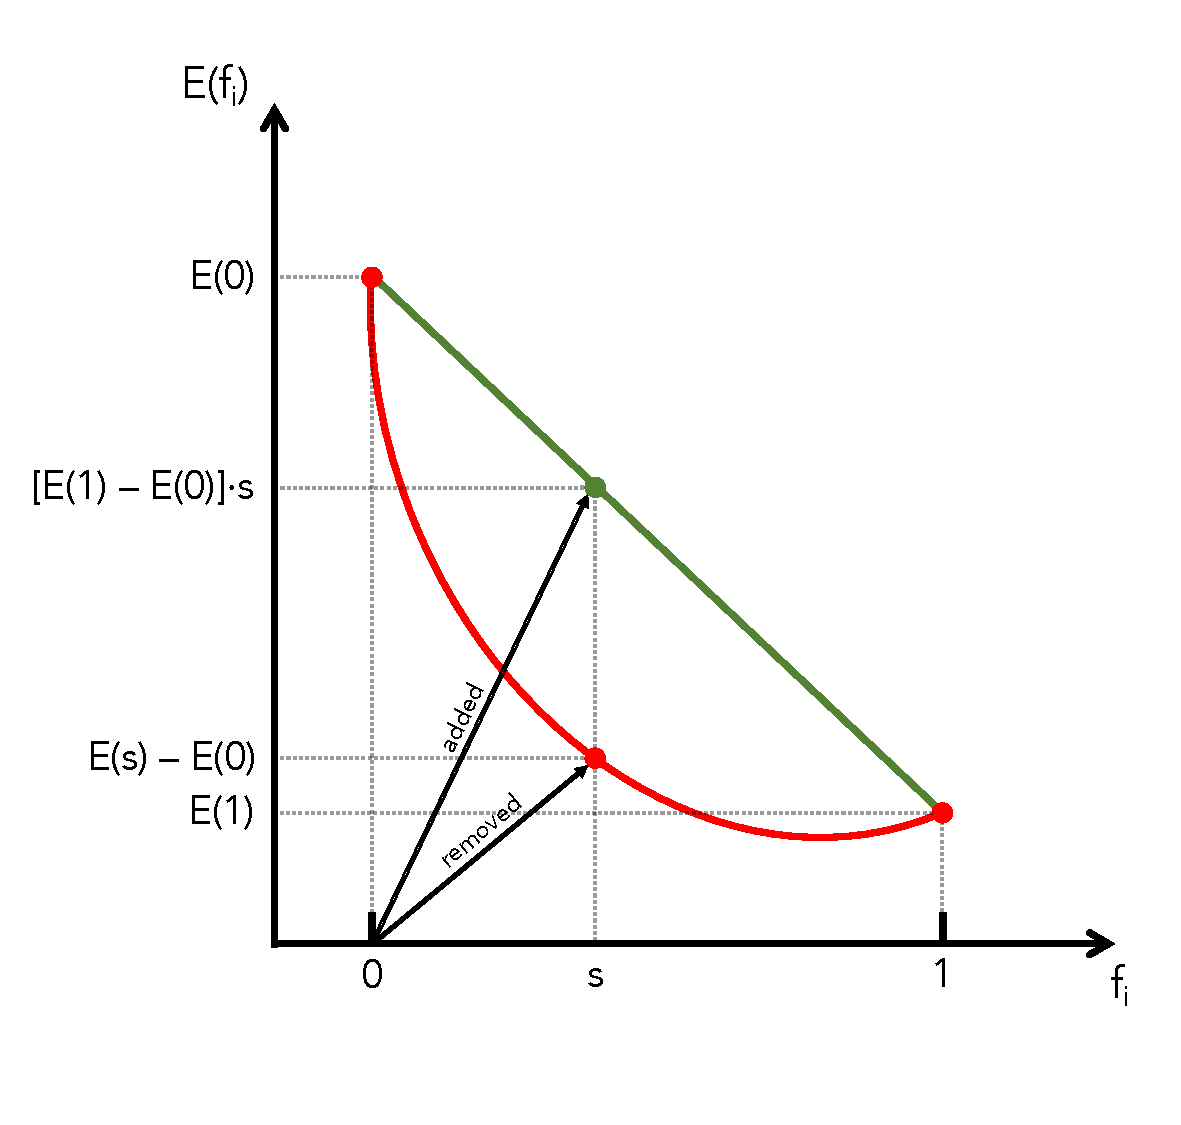
\includegraphics[width=0.7\linewidth]{generalized-pwl.pdf}
    \caption[Graphical representation of the KI correction.]{Visualization of the effects of the KI correction on some local or semi-local density-functional. The red curve represents the energy of some non-linear base functional (e.g. PBE) as a function of the occupation of the $i$-th orbital, while the green curve gives the energy upon the application of the KI correction. At a given value $f_i=s$, KI removes the non-linear term, $E(s)-E(0)$, and adds a linear term given by the total energy difference at $f_i=1$ and $f_i=0$ and calculated at the level of the base functional.}
    \label{fig:kc-correction-visual}
\end{figure}

The expression given in \cref{eq:pi-term-general}, with the choice \eqref{eq:lambda-definition} for $\lambda_i$, defines the so-called \emph{Koopmans integral} (KI) correction \cite{borghi_koopmans-compliant_2014}, since the energy derivative is set to be equal to the integral average of all the values of the derivative at fractional occupations. It is worth to mention that this does not represent the only possible choice for the value of $\lambda_i$: initial works about KC functionals \cite{dabo_non-koopmans_2009,dabo_koopmans_2010,borghi_koopmans-compliant_2014} were considering also the possibility to evaluate the energy derivatives at a specific value $f_{\rm ref}$ of the occupation, e.g. $f_{\rm ref}=1/2$. The problem with this choice is that it requires to guess the value of the optimal occupation number, which in general is system-dependent and, even within a specific system, can vary between different orbitals. The KI correction represents then the conventional way to construct Koopmans functionals, and shortly we will see its application to local DFAs and to the PZ functional.

One of the difficulties with the expression for the $\Pi_i$ terms given in \cref{eq:pi-term-general,eq:lambda-definition} is that it requires, in principle, the knowledge of the values of the (self-consistent) energy $E^{\rm DFT}$ at any $s$ between 0 and 1, which is something that we certainly want to avoid. A simplified version of the KI correction can be obtained by neglecting, in a first moment, the relaxation effects following the change in the occupation of any orbitals. In this way, we can find an expression where only the quantities computed for the $N$-particle system play a role. We recall the expression for the total density given in \cref{eq:janak-density}, and we introduce the orbital densities $\rho_i$ and the occupation-independent orbital densities $n_i$:
%
\begin{equation}
    \begin{gathered}
    \rho_i(\br) = f_i |\phi_i(\br)|^2 , \\
    n_i(\br) = \rho_i^{f_i=1}(\br) = |\phi_i(\br)|^2 .
    \end{gathered}
    \label{eq:orbital-densities}
\end{equation}
%
If the orbitals relaxation is ignored, the one-electron wave functions are left unchanged upon the variation of any occupations. If a given orbital, initially occupied by $f_i$ electrons, is suddenly emptied the total energy can then be written as
%
\begin{equation}
    E(f_i=0) = E[\rho^{f_i=0}] = E[\rho-\rho_i] ;
    \label{eq:unrelaxed-energy-emptied-orbital}
\end{equation}
%
analogously, if the same orbital gets completely filled, the resulting total energy is
%
\begin{equation}
    E(f_i=1) = E[\rho^{f_i=1}] = E[\rho-\rho_i+n_i] .
    \label{eq:unrelaxed-energy-filled-orbital}
\end{equation}
%
The last two equations can be used in \cref{eq:pi-term-general} to find an explicit expression of the \emph{unscreened} KI correction term, which reads as
%
\begin{equation}
    \Pi_i^{\rm uKI}[\rho,\rho_i] = E^{\rm DFT}[\rho - \rho_i] - E^{\rm DFT}[\rho] + f_i \left( E^{\rm DFT}[\rho - \rho_i + n_i] - E^{\rm DFT}[\rho - \rho_i] \right) .
    \label{eq:ki-correction}
\end{equation}
%
and introduces a dependence on the orbital densities. The effects of the orbitals relaxation are then accounted for by scaling the unscreened corrective terms via some scalar, orbital-dependent screening parameters $\alpha_i$; we refer to \cref{sec:screening-parameters} for a detailed description of the methods to compute the screening parameters. By means of the unrelaxed KI correction and of the scalar screening parameters, the fully-screened correction terms appearing in \cref{eq:kc-functional-coarse} are approximated as $\Pi_i^{\rm KI} \approx \alpha_i \Pi_i^{\rm uKI}$, and we finally arrive to \cite{borghi_koopmans-compliant_2014}
%
\begin{equation}
    E^{\rm KI}[\{\rho_i\}] = E^{\rm DFT}[\rho] + \sum_i \alpha_i \Pi_i^{\rm uKI}[\rho, \rho_i] .
    \label{eq:ki-functional}
\end{equation}
%
The proper way of calling the functional in \cref{eq:ki-functional} is KI@DFA -- e.g., if the base functional is LDA or PBE, the corresponding KI-corrected functional should be called KI@LDA, or KI@PBE. However, if the base functional is a local or semi-local density-functional approximation, we normally refer more generically to \cref{eq:ki-functional} as the ``KI functional''.

Another prominent Koopmans functional is KIPZ, which results from the augmentation of a local density-functional via the KIPZ correction:
%
\begin{equation}
    E^{\rm KIPZ}[\{\rho_i\}] = E^{\rm DFT}[\rho] + \sum_i \alpha_i \Pi_i^{\rm uKIPZ}[\rho, \rho_i] ,
    \label{eq:kipz-functional}
\end{equation}
%
where the KIPZ unrelaxed correction is defined as\footnote{Although KIPZ was already introduced in Ref.\cite{borghi_koopmans-compliant_2014}, the following definition of the KIPZ functional was proposed for the first time in Ref.~\cite{borghi_variational_2015}; in \cref{app:ki-kipz}, we show the equivalence between \cref{eq:kipz-correction} and the former definition of the KIPZ correction.}
%
\begin{equation}
    \Pi_i^{\rm uKIPZ}[\rho,\rho_i] = \Pi_i^{\rm uKI}[\rho,\rho_i] - f_i E_{\rm Hxc}[n_i] ,
    \label{eq:kipz-correction}
\end{equation}
%
showing that, in addition to $\Pi_i^{\rm uKI}$, the KIPZ correction contains also a PZ-like SIC term. As as consequence of the presence of such term, KIPZ -- differently from KI -- modifies the energy of the underlying DFT functional even at integer occupations. Indeed, the functional of \cref{eq:kipz-functional} can be seen as a KI correction on top of the screened PZ functional, i.e. KI@$\alpha$PZ. Considering then $\alpha$PZ as the base functional, KIPZ does not change the energy of $\alpha$PZ at integer occupations (as expected by any KI-like correction). In \cref{app:ki-kipz}, we detail this interpretation of the KIPZ functional.

One of the main features that emerges in Koopmans functionals is the ODD character, also present in the PZ functional. This is a consequence of the state-dependent nature of the Koopmans' condition, which cannot be fulfilled by an explicit functional of the density, whereas it requires the introduction of additional degrees of freedom: the orbital densities. Unfortunately, the orbital-density-dependence makes the search of a variational ground state much more complex, as it generally breaks the unitary invariance characterizing standard density-functionals. Some of these issues will be addressed in \cref{sec:variational-procedure}.

\subsection{Screening parameters\label{sec:screening-parameters}}
The effects due to the orbitals relaxation, upon changes in the occupation numbers, must be accounted for in order to have an effective Koopmans correction. While this would generally require a complex treatment of the screening -- e.g., by evaluating the convolution of the inverse dielectric matrix with the Koopmans potential -- here we consider a simplified, yet effective, approach which accounts for the screening via some scalar and orbital-dependent parameters, $\alpha_i$, yielding the following approximation for the fully screened KI correction
%
\begin{equation}
    \Pi_i^{\rm KI} \approx \alpha_i \Pi_i^{\rm uKI} .
    \label{eq:approx-screened-ki}
\end{equation}
%
In the following, we discuss two methods to evaluate the screening parameters: via \emph{finite energy differences}, which requires to compute self-consistent energies at $N \pm 1$ electrons, and from \emph{linear response theory}, which relies on the $N$-particle system only, whereas it introduces a second-order approximation for the $\Pi_i$ terms.

\subsubsection*{Finite differences}
To support the forthcoming discussion, let us consider \cref{fig:pwl-ki-dft}. In panels (a)-(b), the PBE, unscreened KI (uKI), and $\alpha$-screened KI ($\alpha$KI) total energies and eigenvalues are plotted as functions of the orbital occupation. Unsurprisingly, the PBE energy shows a non-linear convex behavior which is almost quadratic, as confirmed by the linear trend of the corresponding eigenvalue. The unscreened Koopmans correction (i.e. $\alpha_i=1$, $\forall i$) significantly reduces the convexity of the PBE energy, whereas it leaves unchanged -- as expected -- the energy at integer occupations. At fractional occupations, uKI displays a non-negligible curvature, as confirmed once again by panel (b), due to the neglect of the relaxation effects. The latter generally lower the energy, therefore the lack of screening produces a uKI \emph{concave} curve which overestimates the fully screened KI energy (which is, by construction, a linear curve connecting the PBE energies at $f_i=0$ and $f_i=1$). Ultimately, the red and blue curves represent the lower and upper bounds, respectively, of the KI functional as a function of the screening parameter. As shown in panel (c), the change of concavity of the energy curve indicates the existence of some optimal $\alpha_i$, for which the left and right derivatives -- i.e. $N$-particle IP and $(N-1)$-particle EA -- match. The idea behind this finite-differences method then, is to exploit this feature to determine the values of the screening parameters.

\begin{figure}
    \centering
    \sbox{\measurebox}{
        \begin{minipage}{.48\linewidth}
            \subfloat[]{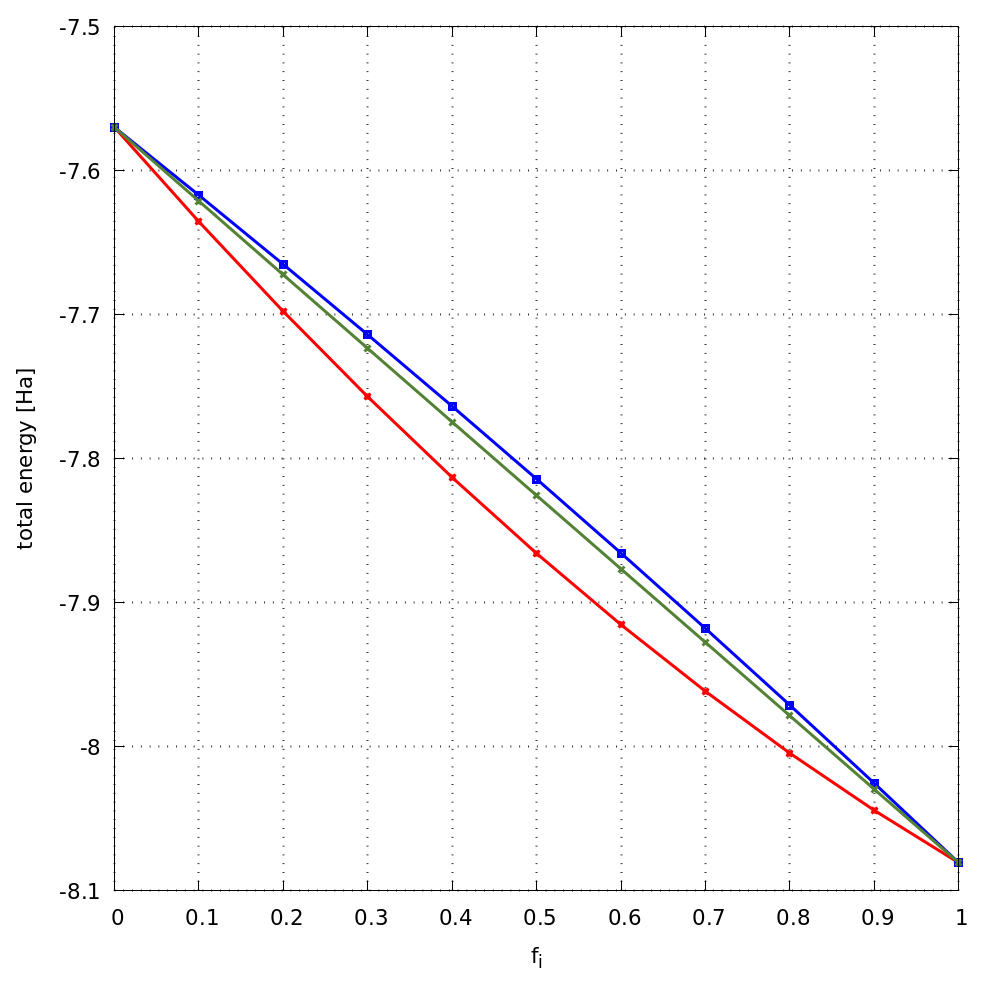
\includegraphics[width=\linewidth]{ene-vs-occ-homo.png}}
        \end{minipage}
    }
    \usebox{\measurebox}
    \begin{minipage}{.48\linewidth}
        \subfloat[]{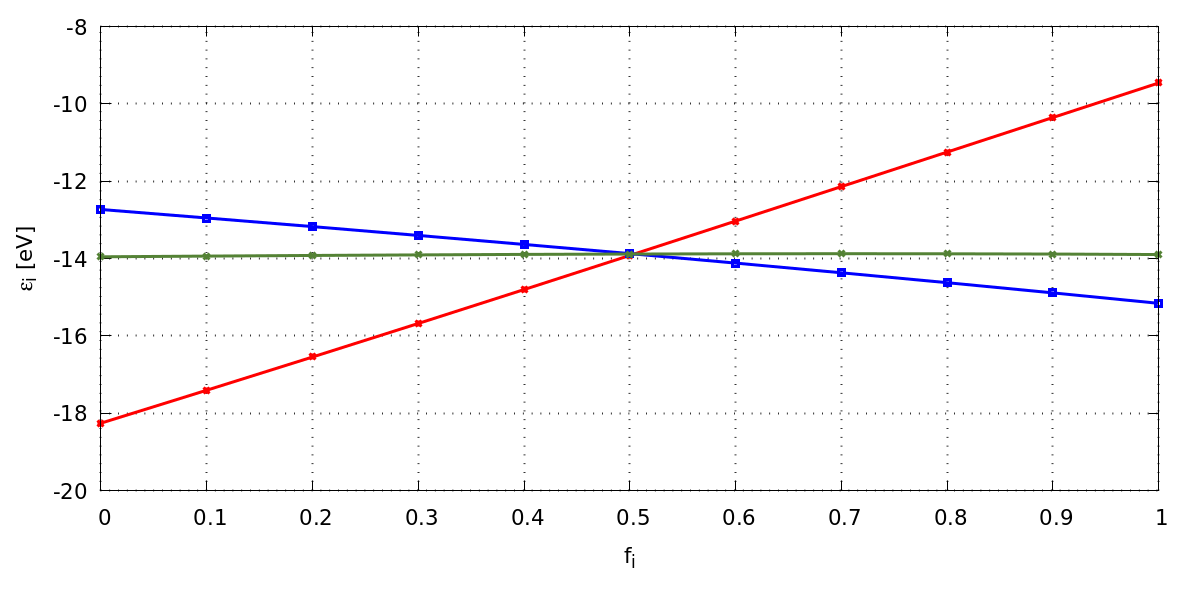
\includegraphics[width=\linewidth]{eig-vs-occ-homo.png}}
        \vfill
        \subfloat[]{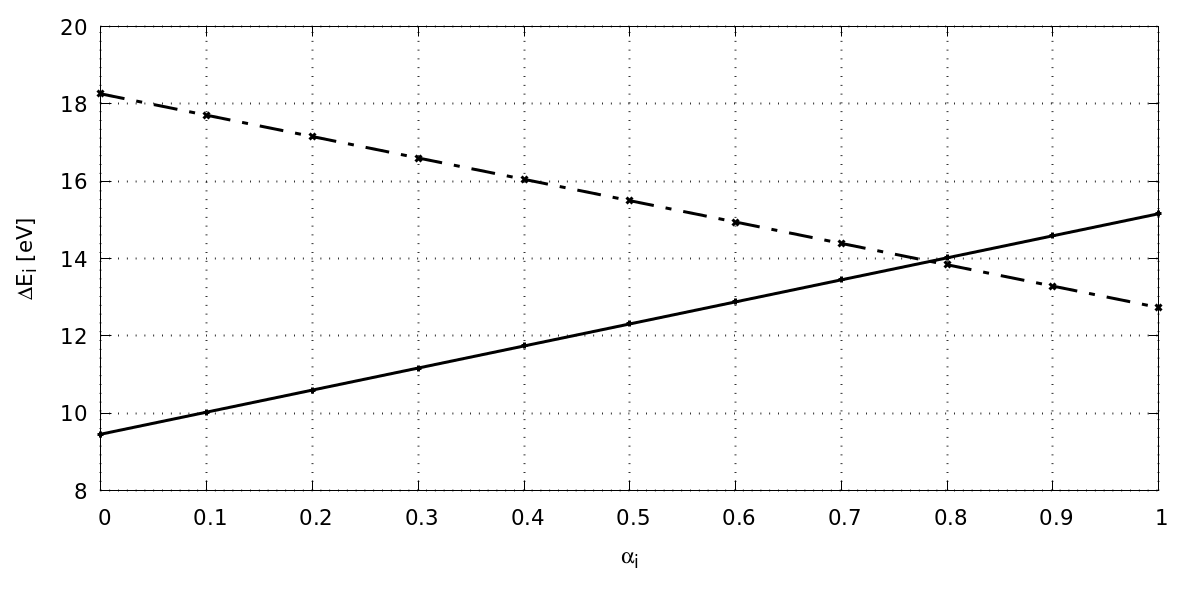
\includegraphics[width=\linewidth]{ip-ea-vs-alpha.png}}
    \end{minipage}
    \caption[Total energy and $\varepsilon_{\rm HO}$ vs. $f_{\rm HO}$ for $CH_4$ molecule]{Total energies (a) and HO eigenvalues (b) calculated at the PBE level (red curve), and from the screened (green curve) and unscreened (blue curve) KI functionals, with respect to the occupation of the HO molecular orbital of the methane molecule; also for the two Koopmans functionals, we considered variations in the occupation of the PBE highest-occupied KS orbital. Panel (c) shows the KI differential IP (continuous line) and EA (dashed line) as functions of the screening parameter: in particular for $\alpha=0$ and $\alpha=1$, the PBE and uKI values, respectively, are retrieved.}
    \label{fig:pwl-ki-dft}
\end{figure}

From \cref{eq:koopmans-condition}, the matching of the differential $N$-particle IP and $(N-1)$-particle EA, translates into the condition
%
\begin{equation}
    \lambda_i^{f_i=1}(\alpha) = \lambda_i^{f_i=0}(\alpha) .
    \label{eq:alpha-dscf-condition}
\end{equation}
%
We emphasize the Koopmans' condition \eqref{eq:koopmans-condition} is strictly fulfilled only the fully-screened functional; as also showed in \cref{fig:pwl-ki-dft}, the unscreened KI functional is not strictly Koopmans-compliant, while -- at good level of approximation -- the $\alpha$-screened KI functional satisfies the Koopmans' condition for the optimal $\alpha$ values. In this sense, \cref{eq:alpha-dscf-condition} can be seen as a way to enforce the Koopmans' condition on the unscreened Koopmans functional. The optimal values of $\alpha$ are found by means of the secant method, described in \cref{fig:secant-method}. At each step, we suppose a linear $\alpha$-dependence of $\lambda_i$ and \cref{eq:alpha-dscf-condition} is solved by
%
\begin{equation}
    \alpha_i^{(n+1)} = \alpha_i^{(n)} \frac{\lambda_i(\alpha_i^{(n+1)}) - \lambda_i(0)}{\lambda_i(\alpha_i^{(n)}) - \lambda_i(0)} .
    \label{eq:alpha-intermediate-expression}
\end{equation}

\begin{figure}
    \centering
    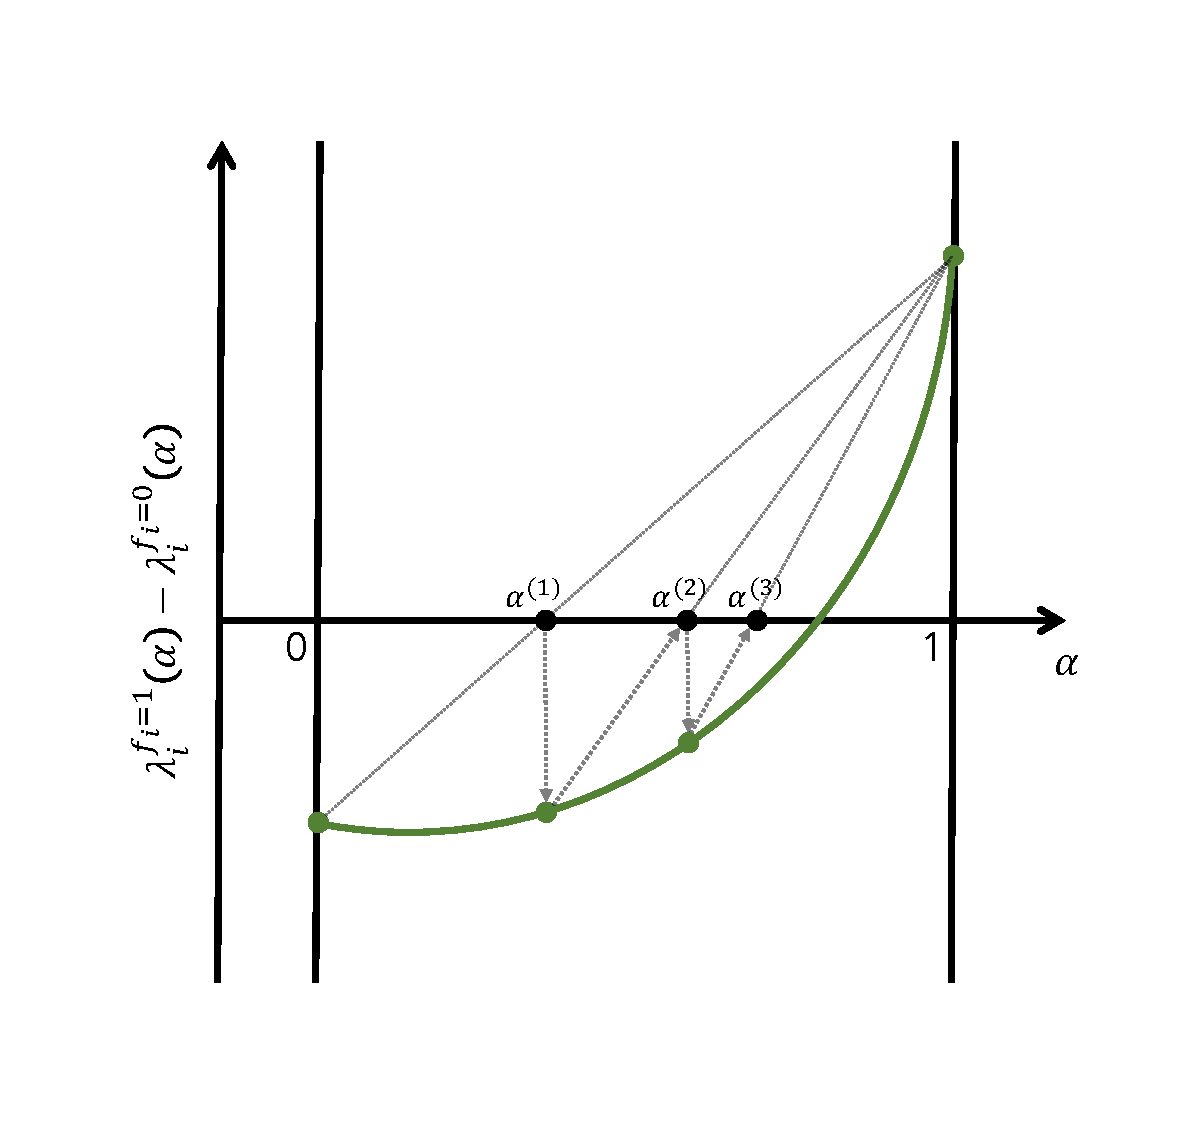
\includegraphics[width=0.63\linewidth]{secant-method.pdf}
    \caption[Secant method to determine the screening parameters]{In order to find the zero of the function $\tau(\alpha) = \lambda_i^{f_i=1}(\alpha) - \lambda_i^{f_i=0}(\alpha)$, the first step is to consider a linear dependence of $\lambda_i$ on $\alpha$, such as the straight line connecting the points at $\alpha=0,1$. Then, after determining the first guess $\alpha^{(1)}$, we can repeat the procedure defining a straight line that connects $\tau(\alpha^{(1)})$ and, e.g., $\tau(1)$, and finding a new guess $\alpha^{(2)}$. For smooth functions, the zero of $\tau(\alpha)$ is numerically found when two consecutive estimations of $\alpha$ provide the same value within the chosen threshold.}
    \label{fig:secant-method}
\end{figure}

The values of $\lambda_i(0)$ and of $\lambda_i(\alpha_i^{(n)})$ can be computed from the expectation value of the DFT and Koopmans Hamiltonians, respectively, over the $i$-th orbital (see also \cref{sec:variational-procedure}). With regards to $\lambda_i(\alpha_i^{(n+1)})$, we can already assume the validity of the Koopmans' condition and express the energy as a linear function of $f_i$:
%
\begin{equation}
    E^{\rm KC}(f_i) \approx E^{\rm KC}(f_{\rm ref}) + \left. \frac{dE^{\rm KC}}{df_i} \right|_{f_{\rm ref}} (f_i-f_{\rm ref}) =
    E^{\rm KC}(f_{\rm ref}) + \lambda_i^{f_i=f_{\rm ref}} \cdot (f_i-f_{\rm ref}) ,
    \label{eq:energy-expansion-lambda}
\end{equation}
%
where $E^{\rm KC}$ refers to a generic Koopmans functional (KI, KIPZ). By matching the two expressions obtained from \cref{eq:energy-expansion-lambda} for $f_{\rm ref} = 0$ and $f_{\rm ref} = 1$, we can write $\lambda_i$ as an energy difference, i.e. $\lambda_i = E^{\rm KC}(f_i=1) - E^{\rm KC}(f_i=0)$, to arrive to the final expression for the screening parameters:
%
\begin{equation}
    \alpha_i^{(n+1)} = \alpha_i^{(n)} \frac{\Delta E^{\rm KC}_i - \braket{\phi_i|\hat{h}^{\rm DFT}|\phi_i}}{\braket{\phi_i|\hat{h}^{\rm KC}|\phi_i} - \braket{\phi_i|\hat{h}^{\rm DFT}|\phi_i}} ,
    \label{eq:screening-parameter-iterative}
\end{equation}
%
where $\Delta E^{\rm KC}_i = E^{\rm KC}(N) - E^{\rm KC}_i(N-1)$ or $\Delta E^{\rm KC}_i = E^{\rm KC}_i(N+1) - E^{\rm KC}(N)$, depending on the nature (occupied or empty) of the orbital. We observe that, given the absence of KI correction at integer electron numbers, $\Delta E^{\rm KC}_i$ reduces to a DFT energy difference for the KI functional, and to a $\alpha$PZ energy difference for the KIPZ functional. Of course such procedure must be repeated for all the orbitals in the system, unless one can expect distinct orbitals to yield similar results (more details about the technicalities behind the calculation of the screening parameters are given in \cref{ch:band-structures}).

\cref{eq:screening-parameter-iterative} was introduced in Ref.~\cite{nguyen_koopmans-compliant_2018}. Previous works were calculating the screening parameters using the same secant method -- with the only technical difference that the linear dependence on $\alpha$ was directly imposed on $\tau(\alpha)$ (see caption of \cref{fig:secant-method}), rather than on $\lambda_i^{f_i=1}(\alpha)$ and $\lambda_i^{f_i=0}(\alpha)$ separately -- and were not imposing \cref{eq:energy-expansion-lambda}. The two methods can be considered equivalent, as the only difference in the present approach is that it is possible to replace some derivatives with a difference of total energies.

\begin{figure}
    \centering
    \subfloat[]{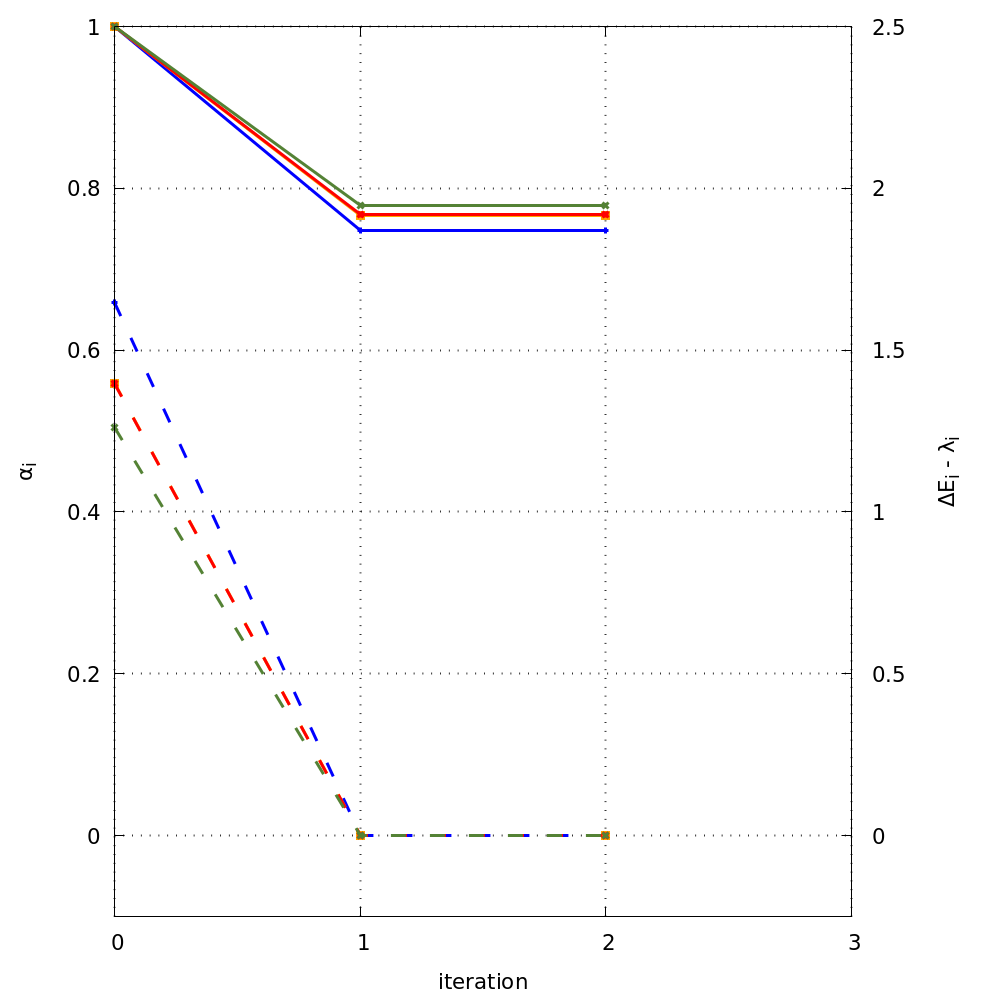
\includegraphics[width=0.4\linewidth]{alpha_ki_conv.png}} \qquad
    \subfloat[]{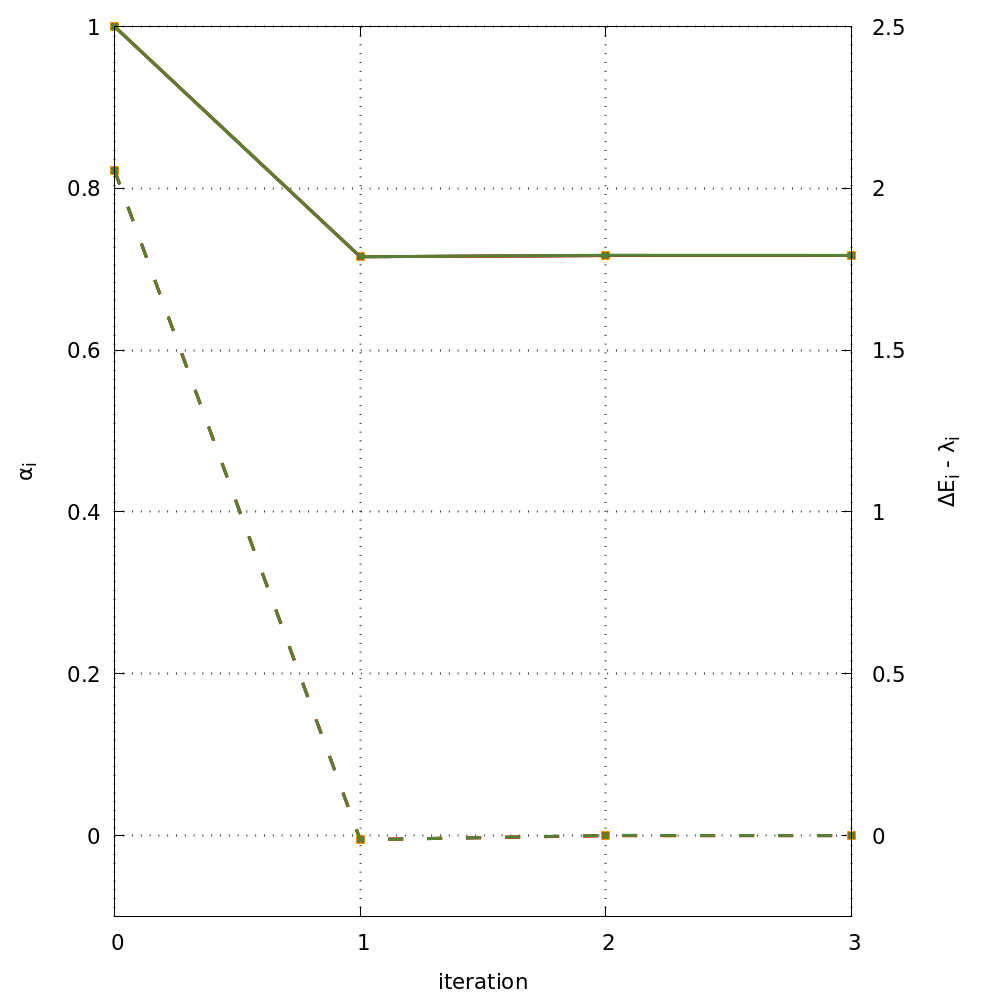
\includegraphics[width=0.4\linewidth]{alpha_kipz_conv.png}}
    \caption[Convergence of screening parameters]{Convergence study of the screening parameters for the four valence orbitals of the methane molecule, computed at the KI (left panel) and KIPZ (right panel) levels. The dashed lines give a measure of the deviation from the PWL, i.e. $\Delta E_i - \lambda_i$. The orbitals used in the KI calculation are the KS ones (two of which are almost identical) and the corresponding screening parameters are converged already at the end of the first iteration; for KIPZ, the screening parameters refer to the KIPZ variational orbitals (see \cref{sec:variational-procedure}) -- all symmetrically equivalent -- and converge within the chosen threshold ($10^{-3}$) in two iterations, although the first estimation provides results which agree with the fully converged ones within 0.02 eV.}
    \label{fig:alphas-convergence}
\end{figure}

To end this section, we mention that, although the dependence of $\lambda_i$ on $\alpha$ is generally unknown, most of the times it displays an almost linear trend. As a consequence, the value of $\alpha$ at the first iteration proved to be extremely close to the final solution (see \cref{fig:alphas-convergence}), especially if initialized with some good guess of $\alpha$. In actual calculations then, we often consider the screening parameters obtained after a single iteration, starting from the most reasonable physical guess: the inverse of the dielectric constant, $\alpha_i^{(0)} = \epsilon^{-1}$,
%
\begin{equation}
    \alpha_i = \epsilon^{-1} \frac{\Delta E^{\rm KC}_i - \braket{\phi_i|\hat{h}^{\rm DFT}|\phi_i}}{\braket{\phi_i|\hat{h}^{\rm KC}|\phi_i} - \braket{\phi_i|\hat{h}^{\rm DFT}|\phi_i}} .
    \label{eq:screening-parameter-dscf}
\end{equation}

\subsubsection*{Linear response}
As the screening parameters account for the relaxation effects following a change in the orbitals occupations (process that can be assimilated to the presence of some perturbing potential), it is quite reasonable to assimilate them to the system's response to some external perturbation. Following this idea, Colonna and collaborators ~\cite{colonna_screening_2018} found an alternative definition for the screening parameters, which turns out to be exact up to a second-order expansion of the Koopmans correction. Hereafter we report the demonstration showed in Ref.~\cite{colonna_screening_2018}.

Let us consider the fully-relaxed KI correction given in \cref{eq:pi-term-general}, and express it as
%
\begin{equation}
    \Pi_i^{\rm KI}(f_i) = E^{\rm DFT}[\rho^{f_i=0}] - E^{\rm DFT}[\rho] + f_i \left( E^{\rm DFT}[\rho^{f_i=1}] - E^{\rm DFT}[\rho^{f_i=0}] \right) ;
    \label{eq:full-ki-correction-relaxed}
\end{equation}
%
the expression above closely resembles \cref{eq:ki-correction}, however, it is important to highlight that while \cref{eq:full-ki-correction-relaxed} is exact as it does not make any assumption on the energies at different occupations, the form of \cref{eq:ki-correction} results from the assumption of frozen-orbitals, which allows to rewrite the energies in terms of the orbitals of the neutral system (e.g., $E[\rho^{f_i=0}] = E[\rho-\rho_i]$). If we consider now a second-order Taylor expansion for the DFT energy as a function of $f_i$ around some reference occupation $f_{\rm ref}$ -- essentially the expansion of \cref{eq:energy-expansion-lambda} where we include also the quadratic term -- the KI correction takes the following form:
%
\begin{equation}
    \begin{split}
    \Pi_i^{\rm KI}(f_i) =\
    %
    &E^{\rm DFT}[\rho^{f_i=f_{\rm ref}}] - f_{\rm ref} \left. \frac{dE^{\rm DFT}}{df_i} \right|_{f_{\rm ref}} + \frac{1}{2} f_{\rm ref}^2 \left. \frac{d^2 E^{\rm DFT}}{df_i^2} \right|_{f_{\rm ref}} - \\
    %
    &E^{\rm DFT}[\rho^{f_i=f_{\rm ref}}] - (f_i - f_{\rm ref}) \left. \frac{dE^{\rm DFT}}{df_i} \right|_{f_{\rm ref}} - \frac{1}{2} (f_i - f_{\rm ref})^2 \left. \frac{d^2 E^{\rm DFT}}{df_i^2} \right|_{f_{\rm ref}} + \\
    %
    &f_i \Bigg\{ E^{\rm DFT}[\rho^{f_i=f_{\rm ref}}] + (1 - f_{\rm ref}) \left. \frac{dE^{\rm DFT}}{df_i} \right|_{f_{\rm ref}} - \frac{1}{2} (1 - f_{\rm ref})^2 \left. \frac{d^2 E^{\rm DFT}}{df_i^2} \right|_{f_{\rm ref}} - \\
    %
    &E^{\rm DFT}[\rho^{f_i=f_{\rm ref}}] + f_{\rm ref} \left. \frac{dE^{\rm DFT}}{df_i} \right|_{f_{\rm ref}} - \frac{1}{2} f_{\rm ref}^2 \left. \frac{d^2 E^{\rm DFT}}{df_i^2} \right|_{f_{\rm ref}} \Bigg\} + \mathcal{O}\left( (f_i - f_{\rm ref})^3 \right) \\
    %
    =\ &\frac{1}{2} f_i(1-f_i) \left. \frac{d^2 E^{\rm DFT}}{df_i^2} \right|_{f_i=f_{\rm ref}} + \mathcal{O}\left( (f_i - f_{\rm ref})^3 \right) .
    \end{split}
    \label{eq:ki-correction-second-order}
\end{equation}
%
At this point, by means of Janak's and Hellmann-Feynman theorems, we can write the second-order derivative of the energy as
%
\begin{equation}
    \begin{split}
    \frac{d^2 E^{\rm DFT}}{df_i^2} &= \frac{d\varepsilon_i}{df_i} = \braket{\psi_i|\frac{d\hat{v}_{\rm KS}}{df_i}|\psi_i} \\
    &= \int d\br d\br' n_i(\br) \frac{\delta v_{\rm KS}([\rho],\br)}{\delta\rho(\br')} \frac{d\rho(\br')}{df_i} ,
    \end{split}
    \label{eq:second-derivative-energy}
\end{equation}
%
where $\psi_i$ are the KS states, and the derivative of the KS potential yields the Hxc kernel, $f_{\rm Hxc}(\br,\br')$. The derivative of the density with respect to the orbital occupations is less trivial and requires further manipulations; by recalling the definition of the density \eqref{eq:janak-density}, we can write the its derivative as
%
\begin{equation}
    \begin{split}
    \frac{d\rho(\br)}{df_i} &= n_i(\br) + \sum_j f_j \frac{dn_j(\br)}{df_i} \\
    &= n_i(\br) + \sum_j f_j \int d\br' \frac{\delta n_j(\br)}{\delta v_{\rm KS}(\br')} \frac{dv_{\rm KS}(\br')}{df_i} .
    \end{split}
    \label{eq:density-derivative-1}
\end{equation}
%
By introducing the non-interacting density-density response function $\chi_0(\br,\br')$\footnote{$\chi_0$ gauges the \emph{neutral} response of the system, namely the part of the response which does not involve any changes in the particle number: i.e. $\chi_0(\br,\br') = \left. \frac{\delta\rho(\br)}{\delta v_{\rm KS}(\br')} \right|_{\{ f_i \} = {\rm const}}$.} and adding another chain of derivatives, \cref{eq:density-derivative-1} takes the form of a Dyson-like equation for the derivative of the density:
%
\begin{equation}
    \begin{split}
    \frac{d\rho(\br)}{df_i} &= n_i(\br) + \int d\br' d\br'' \chi_0(\br,\br') \frac{\delta v_{\rm KS}(\br')}{\delta \rho(\br'')} \frac{d\rho(\br'')}{df_i} \\
    &= n_i(\br) + \int d\br' [\chi_0 f_{\rm Hxc}](\br,\br') \frac{d\rho(\br')}{df_i} ,
    \end{split}
    \label{eq:density-derivative-2}
\end{equation}
%
where the notation $[\chi_0 f_{\rm Hxc}]$ indicates the contraction of the two quantities. \cref{eq:density-derivative-2} can be recast in a linear expression (for the derivative of the density), by introducing the interacting polarizability $\chi(\br,\br')$ -- solution of the Dyson equation $\chi = \chi_0 + \chi_0 f_{\rm Hxc} \chi$. Eventually, this allows to express the density variations in terms of the dielectric matrix:
%
\begin{equation}
    \begin{split}
    \frac{d\rho(\br)}{df_i} &= n_i(\br) + \int d\br' [\chi f_{\rm Hxc}](\br,\br') n_i(\br') \\
    &= \int d\br' \left\{ \delta(\br-\br') + [\chi f_{\rm Hxc}](\br,\br') \right\} n_i(\br') \\
    &= \int d\br' \epsilon^{-1}(\br,\br') n_i(\br') ,
    \end{split}
    \label{eq:density-derivative-final}
\end{equation}
%
where we introduced $\epsilon^{-1} = 1 + \chi f_{\rm Hxc}$. By putting together Eqs.~\eqref{eq:ki-correction-second-order}, \eqref{eq:second-derivative-energy} and \eqref{eq:density-derivative-final}, we obtain the following expression -- up to second-order -- for the fully-relaxed KI correction
%
\begin{equation}
    \Pi_i^{\rm KI(2)}(f_i) = \frac{1}{2} f_i(1-f_i) \int d\br d\br' [\epsilon^{-1} f_{\rm Hxc}](\br,\br') n_i(\br) n_i(\br') ;
    \label{eq:relaxed-ki-second-order}
\end{equation}
%
a similar expression can be obtained for $\Pi_i^{\rm uKI(2)}$, where the lack of relaxation effects reduces the dielectric matrix to the identity -- the second term on the right-hand side of \cref{eq:density-derivative-1} indeed disappears, leaving only the contribution from the explicit derivative $\partial E / \partial f_i$. Finally, by defining the screening parameter as the ratio between the relaxed and the unrelaxed KI correction -- as for \cref{eq:approx-screened-ki} -- we obtain the following second-order expression:
%
\begin{equation}
    \alpha_i = \frac{\int d\br d\br' [\epsilon^{-1} f_{\rm Hxc}](\br,\br') n_i(\br) n_i(\br')}{\int d\br d\br' f_{\rm Hxc}(\br,\br') n_i(\br) n_i(\br')} .
    \label{eq:screening-parameter-dfpt}
\end{equation}
%
We observe that, by approximating $\epsilon^{-1}(\br,\br')$ to a constant, $\alpha_i$ reduces to the inverse of the dielectric constant, which further legitimizes the choice made in \cref{eq:screening-parameter-dscf} for the 0-th order screening parameter.

In practice, the screening parameter of \cref{eq:screening-parameter-dfpt} can be calculated resorting to the linear-response approach of density-functional perturbation theory (DFPT) \cite{colonna_screening_2018}. The knowledge of the (interacting) density-density response function, $\chi$, allows to compute the integral on the right-hand side of the first line of \cref{eq:density-derivative-final}. The only limitation of this approach is that it requires the knowledge of the second derivatives -- i.e. the kernel -- of the base functional: while for KI corrections on top of standard DFAs, such as LDA or PBE, such derivatives are known and already implemented in most of the electronic-structure codes, for KIPZ computing the kernel is not a straightforward task and the DFPT approach -- for the moment -- does not apply. To highlight the agreement between with the finite-differences method, in \cref{fig:alphas-dscf-dfpt} we compared the screening parameters for the orbitals of the methane molecule: the effect of the small differences observed is not significant for the final eigenvalues, which agree within 0.1~eV. 

\begin{figure}
    \centering
    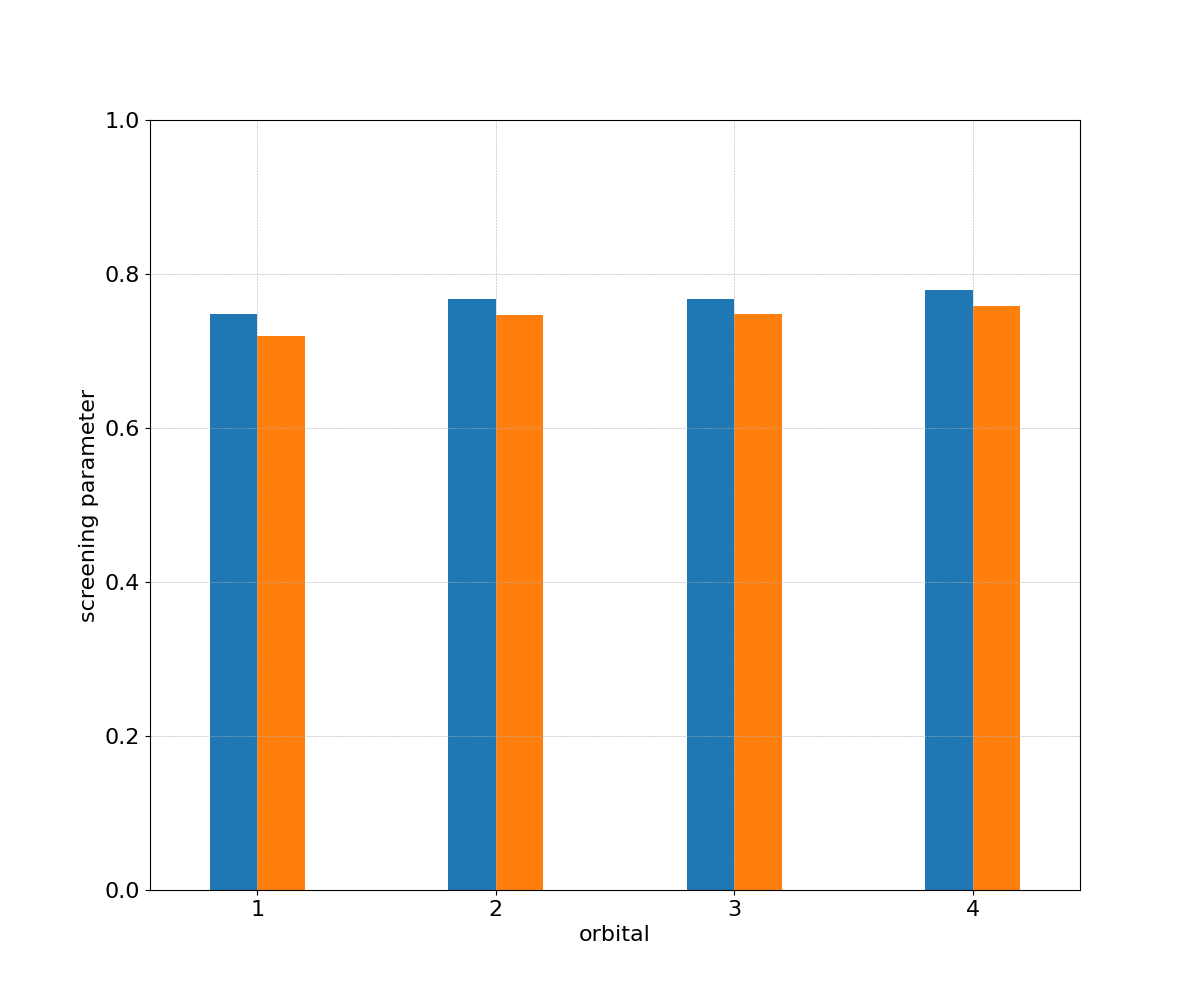
\includegraphics[width=0.6\linewidth]{alphas_dscf_dfpt.png}
    \caption[Comparison of screening parameters from $\Delta$SCF and DFPT]{Screening parameters for the four KS-PBE valence orbitals of ${\rm CH}_4$ computed from finite differences (blue) and from the linear-response method (orange).}
    \label{fig:alphas-dscf-dfpt}
\end{figure}

\subsection{Variational procedure\label{sec:variational-procedure}}
Similarly to PZ-SIC, Koopmans functionals are considered as an extension of standard DFT functionals, for which we can assume the existence of a variational principle. Unfortunately, the ODD nature of Koopmans functionals makes the minimization procedure more complex than in density-functionals: the latter depend solely on the total density, therefore any sets of orbitals connected by unitary transformations are energetically equivalent, while ODD functionals break such unitary invariance -- i.e. they generally yield different energies for distinct representations, even when they span the same subspace. As a consequence, in addition to the search for the optimal subspace $\hat{\rho}$, the minimization of an ODD functional requires scanning over all the representations that span $\hat{\rho}$:
%
\begin{equation}
    E^{\rm KC}_0 = \min_{\hat{\rho}} \min_{\{ \phi_i \}_{\hat{\rho}}} \bigg\{ E^{\rm KC}[\{ \rho_i \}] + \sum_{ij} \Lambda_{ij} (\braket{\phi_i|\phi_j} - \delta_{ij}) \bigg\} ,
    \label{eq:minimization-koopmans}
\end{equation}
%
where $E^{\rm KC}$ represents a generic Koopmans functional -- we remark that the described procedure applies to any ODD approach, including the PZ functional -- and the Lagrange multipliers $\Lambda_{ij}$ ensure the orthonormality of the set of one-electron wave functions $\{ \phi_i \}$. The Euler-Lagrange equations associated to the minimization problem of \cref{eq:minimization-koopmans} are
%
\begin{equation}
    \hat{h}^{\rm KC}_i \ket{\phi_i} = \sum_j \Lambda_{ij} \ket{\phi_j} ,
    \label{eq:euler-lagrange-koopmans}
\end{equation}
%
where $\hat{h}^{\rm KC}_i$ is the ODD Hamiltonian associated to the $i$-th orbital, defined as
%
\begin{equation}
    \begin{split}
        \hat{h}^{\rm KC}_i \equiv \hat{h}^{\rm KC}[\rho,\rho_i] &= \frac{\delta E^{\rm KC}[\{ \hat{\rho}_i \}]}{\delta \rho_i} \\
        &=  \hat{h}^{\rm DFT}[\rho] + \alpha_i \hat{v}^{\rm KC}_i
    \end{split}
    \label{eq:koopmans-functional-derivative}
\end{equation}
%
and $\hat{v}_i^{\rm KC}$ is the ODD potential
%
\begin{equation}
    \hat{v}^{\rm KC}_i \equiv \hat{v}^{\rm KC}[\rho,\rho_i] = \sum_j \frac{\delta \Pi_j^{\rm KC}[\rho,\rho_j]}{\delta \hat{\rho}_i} .
    \label{eq:koopmans-ith-potential}
\end{equation}
%
As a result of the ODD nature of Koopmans functionals, the energy derivatives are also orbital-density-dependent, which means that for each vector $\phi_i$ there is a different potential acting on it. As showed in \cref{sec:koopmans-hamiltonian}, this complication does not impede to define a unique -- although non-local -- operator whose representation over the vectors $\{ \phi_i \}$ matches the matrix of Lagrange multipliers introduced in \cref{eq:euler-lagrange-koopmans}.

Let us consider now a unitary transformation $U$ within the subspace $\hat{\rho}$, which maps the set of orbitals $\{ \phi_i \}$ into a new set $\{ \phi_i' \}$. We express such transformation in the exponential form $e^A$, with $A$ being an anti-hermitian matrix. Since we are interested in small energy variations, we can assume $A$ to be very small and expand $U$ at the first order
%
\begin{equation}
    U \approx 1 + A ,
    \label{eq:infinitesimal-unitary}
\end{equation}
%
which brings to the following expression for the vectors in the new basis set
%
\begin{equation}
    \begin{gathered}
    \phi_i'(\br) \approx \phi_i(\br) + \sum_j A_{ji} \phi_j(\br) ,\\
    \rho_i'(\br) \approx \rho_i(\br) + \sum_j \left( A_{ji} \phi_i^*(\br) \phi_j(\br) - A_{ij} \phi_j^*(\br) \phi_i(\br) \right) .
    \end{gathered}
    \label{eq:infinitesimal-unitary-orbitals}
\end{equation}
%
The derivative of the energy with respect to any transformation that preserves the anti-hermitian character of $A$ (which, in turn, guarantees the unitarity of $U$) reads as
%
\begin{equation}
    \begin{split}
    \frac{\partial E^{\rm KC}}{\partial A_{jk}} &= \frac{\partial E^{\rm DFT}}{\partial A_{jk}} + \frac{\partial \left( \sum_i \Pi^{\rm KC}_i \right)}{\partial A_{jk}} \\
    &= \sum_{m} \int d\br \frac{\delta \left( \sum_i \Pi^{\rm KC}_i \right)}{\delta \rho_m'(\br)} \frac{\partial \rho_m'(\br)}{\partial A_{jk}} \\
    &= \int d\br \phi_k^*(\br) [ v^{\rm KC}_k(\br) - v^{\rm KC}_j(\br) ] \phi_j(\br) .
    \end{split}
    \label{eq:energy-der-unitary}
\end{equation}
%
\cref{eq:energy-der-unitary} provides an important property holding at the stationary points of a Koopmans functional, and actually of any PZ-like ODD functional, known as the \emph{Pederson condition}:
%
\begin{equation}
    \braket{\phi_k | \hat{v}^{\rm KC}_k | \phi_j} = \braket{\phi_k | \hat{v}^{\rm KC}_j | \phi_j} .
    \label{eq:pederson-condition}
\end{equation}
%
The Pederson condition shows that the matrix of Lagrange multipliers is generally non-hermitian, and becomes hermitian only for the stationary points of the Koopmans energy.

One of the drawbacks due to the lack of unitary invariance, is that it is not possible to resort to the self-consistent diagonalization method used to minimize standard DFT functionals. The ground state can be found via a direct minimization of the energy functional, which is normally more computationally demanding than standard iterative approaches. Within this framework, an effective strategy -- which follows the ensemble-DFT approach for the minimization of the free energy \cite{marzari_ensemble_1997} -- consists of splitting each iteration of the minimization procedure in two steps: an \emph{outer loop}, and an \emph{inner loop} \cite{borghi_variational_2015,stengel_self-interaction_2008,klupfel_optimization_2012}. In the \emph{outer loop}, the orbitals fluctuations lie in the orthogonal space of $\hat{\rho}$\footnote{Here $\hat{\rho}$ is intended to be the subspace spanned by the orbitals at each iteration: e.g., at the $n$-th iteration, if $\{ \phi_i^{(n)} \}$ is the latest set of orbitals computed, the subspace is $\hat{\rho} = \hat{\rho}^{(n)} = \sum_i f_i^{(n)} \ket{\phi_i^{(n)}}\bra{\phi_i^{(n)}}.$}, following the direction determined by, e.g., steepest-descent or conjugate-gradient algorithms; this is essentially the outer minimum of \cref{eq:minimization-koopmans}, and normally requires a re-orthonormalization of the orbitals at each iteration. During the \emph{inner loop} instead, the orbitals are optimized within the current subspace $\hat{\rho}$, and the search is constrained to the domain of unitary transformations; this step corresponds to the inner minimum of \cref{eq:minimization-koopmans}. We remark that the whole procedure is usually performed in the space of complex orbitals \cite{klupfel_importance_2011,lehtola_complex_2016}.

Another important peculiarity that concerns ODD functionals is the emergence of two special representations: the \emph{variational} (or \emph{minimizing}) \emph{orbitals}, which are those that minimize the energy functional, and the \emph{canonical orbitals}, which correspond to the eigenvectors of the matrix of Lagrange multipliers (at the functional minimum). Such distinction becomes necessary as a consequence of the breaking of the unitary invariance, whereas the energy associated to the canonical orbitals (which are a rotation of the variational ones) is generally higher than the variational energy. The situation is of course different from that of unitary-invariant methods, where any set of orbitals yielding the ground-state density minimizes the energy functional.

Moreover, the duality of variational and canonical orbitals introduces an ambiguity in the choice of the quantities that should be interpreted as quasiparticle energies. On one hand, we have that the Koopmans' condition is realized by the orbitals used within the functional. This means that, at the ground state, the Koopmans' condition is satisfied (only) by the variational orbitals. Then, to be consistent with \cref{eq:koopmans-condition}, we should consider the diagonal elements of the matrix of Lagrangian multipliers -- i.e. the $\lambda_i$ terms -- as quasiparticle energies \cite{vydrov_tests_2007}. On the other hand, since at the minimum $\Lambda$ is hermitian, it is reasonable to interpret its eigenvalues as quasiparticle energies. As highlighted by Stengel and Spaldin \cite{stengel_self-interaction_2008}, in PZ functionals this second choice is supported by the fact that: (i) the HO eigenvalue of the PZ Hamiltonian drives the asymptotic decay of the density [see \cref{eq:exp-decay-density}], and therefore it has an actual physical meaning, and (ii) the density of states (DOS) computed from the eigenvalues resembles more closely the KS-DFT DOS, whose profile usually agrees very well with quasiparticle spectra. We remark that, this is probably a consequence of the fact that the KS Hamiltonian embodies the symmetries of the system, which is usually reflected by its eigenvalues (i.e. they possess the right degeneracies). The same, in general, cannot be said for the diagonal elements of the Lagrangian multipliers matrix which, eventually, can bring to a totally misleading spectrum. An example supporting this argument is given by the methane molecule, where the Koopmans (or PZ) variational orbitals are totally equivalent and have identical matrix elements, yielding a single-peak spectrum. For all these reasons, in this thesis, as well as in other previous works treating Koopmans functionals, we share the choice of Stengel and Spaldin and interpret the eigenvalues of the Lagrangian multipliers matrix as quasiparticles.

Finally, we mention that, due to the lack of treatment in the theory of off-diagonal occupations $f_{ij}$, we are constrained to remain in a diagonal representation of the occupation number matrix. While this represents just a technical limitation in insulating systems, where the occupied and empty manifolds are well separated, it prevents from applying Koopmans functionals to metallic systems. A more detailed description of the problem is given in \cref{app:koopmans-metals}.

\subsubsection*{About the minimization of the KI functional}
With regard to the minimization procedure, the KI functional requires further discussion. Although the KI correction does not modify the energy of the underlying base functional at integer occupations, the energy derivatives -- i.e. the orbital-dependent potentials -- are generally different. In \cref{app:ki-kipz}, we report the full expression of the KI potential where, in the limit of insulating systems at zero temperature, we obtain a scalar quantity [see \cref{eq:ki-pot-occ}]. The KI correction then, does not modify the gradient with respect to fully-occupied orbital densities, and its only effect is that of shifting downward the DFT eigenvalues. In other words, the KI energy of the occupied manifold is unitary-invariant, and it does not allow to solve the ambiguity in the choice of the variational orbitals. A way to avoid this issue was proposed in Ref.~\cite{borghi_koopmans-compliant_2014}, where the KI functional is defined as a KIPZ functional with an infinitesimal PZ-SIC term, i.e.
%
\begin{equation}
    E^{\rm KI}[\{ \rho_i \}] \approx E^{\rm KI}[\{ \rho_i \}] - \gamma \sum_i E_{\rm Hxc}[n_i]
    \qquad \text{with} \qquad \gamma \longrightarrow 0 .
    \label{eq:ki-limit-kipz}
\end{equation}
%
The PZ-SIC term breaks the unitary-invariance of the energy without modifying significantly the KI (or DFT) energy, and allows to determine a set of variational orbitals.

We highlight that this issue appears only for proper KI functionals, namely KI corrections on top of local or semi-local DFAs, whereas for KIPZ there is no such ambiguity. Although KIPZ can still be seen as a KI correction, its base functional is the PZ functional, which already breaks the invariance with respect to unitary transformations and offers a way to determine the set of variational orbitals. Eventually, the KI functional requires the stratagem of \cref{eq:ki-limit-kipz}, only if the base functional is unitary-invariant, and only at zero temperature -- in fact, as soon as the temperature raises, some of the orbitals get only partially occupied and non-scalar contributions arise in the KI potential [see Eqs.~\eqref{eq:ki-pot-1}-\eqref{eq:ki-pot-real}].

\subsection{The Koopmans Hamiltonian\label{sec:koopmans-hamiltonian}}
In this section, we propose a definition of the Koopmans Hamiltonian (introduced for the first time in Ref.~\cite{de_gennaro_blochs_2022}), which will turn out to be particularly useful when, in \cref{ch:koopmans-periodic}, we will discuss the validity of the Bloch's theorem in the context of ODD functionals. Below we introduce a unique operator for the Koopmans potential, knowing that this readily extends to the Koopmans Hamiltonian.

As we saw in \cref{sec:variational-procedure}, differently from standard DFT, where the gradient yields a unique operator for any vectors in the Hilbert space, in ODD functionals the Euler-Lagrange equations associated to the minimization problem \eqref{eq:minimization-koopmans} introduce -- rather than one -- a collection of (local and hermitian) operators $\{ \hat{v}_i^{\rm KC} \}$, each of which acts on a specific orbital $\phi_i$. In other words, the action of the Koopmans potential depends on the wave function to which it is applied. Notwithstanding this complication, it is possible to define a unique \emph{non-local} operator, thanks to the fact that for each operator $\hat{v}_i^{\rm KC}$ \emph{only} its action on the corresponding orbital $\phi_i$ is considered; the Koopmans potential then reads as
%
\begin{equation}
    \hat{v}^{\rm KC}[\{ \rho_i \}] = \sum_i \hat{v}^{\rm KC}_i \ket{\phi_i} \bra{\phi_i} ,
    \label{eq:koopmans-potential}
\end{equation}
%
where the expression on the right-hand side must be considered a whole object that cannot be split: in particular, the quantity $\hat{v}^{\rm KC}_i \ket{\phi_i}$ should be considered as a single entity, i.e. a vector $\ket{\Tilde{\phi}_i}$, thus no operator, including identities, can be inserted in between. This detail is fundamental, as it guarantees that each ODD potential $\hat{v}^{\rm KC}_i$ always acts on the orbital from which it has been defined.

Let us consider the pair of states $\psi$ and $\phi$ and compute the degree of hermiticity of $\hat{v}^{\rm KC}$, defined as the difference between the operator and its adjoint. By expressing the two vectors on the basis vecotrs $\{ \phi_i \}$, we obtain
%
\begin{equation}
    \begin{split}
    \braket{\psi|\hat{v}^{\rm KC} - (\hat{v}^{\rm KC})^{\dagger}|\phi} &= \sum_{jk} a_j^* b_k \braket{\phi_j|\hat{v}^{\rm KC} - (\hat{v}^{\rm KC})^{\dagger}|\phi_k} \\
    &= \sum_{jk} a_j^* b_k \sum_i \left( \braket{\phi_j|\hat{v}_i^{\rm KC}|\phi_i}\braket{\phi_i|\phi_k} - \braket{\phi_j|\phi_i}\braket{\phi_i|\hat{v}_i^{\rm KC}|\phi_k} \right) \\
    &= \sum_{jk} a_j^* b_k \left( \braket{\phi_j|\hat{v}_k^{\rm KC}|\phi_k} - \braket{\phi_j|\hat{v}_j^{\rm KC}|\phi_k} \right) ,
    \end{split}
    \label{eq:hermiticity-koopmans-potential}
\end{equation}
%
where $\{ a_j \}$ and $\{ b_k \}$ are the coefficients of $\psi$ and $\phi$, respectively, on the basis $\{ \phi_i \}$, and on the second line we used the fact that the potentials $\hat{v}_i^{\rm KC}$ are hermitian. The right-hand side of \cref{eq:hermiticity-koopmans-potential} is zero whenever the Pederson condition \eqref{eq:pederson-condition} is fulfilled. Therefore, as anticipated in the previous section, the Pederson condition turns into a condition of hermiticity for the Koopmans potential defined in \cref{eq:koopmans-potential}. The same properties readily apply to the Koopmans Hamiltonian
%
\begin{equation}
    \hat{h}^{\rm KC} = \sum_i \hat{h}_i^{\rm KC} \ket{\phi_i} \bra{\phi_i} ,
    \label{eq:koopmans-hamiltonian}
\end{equation}
%
where $\hat{h}_i^{\rm KC} = \hat{h}^{\rm DFT} + \alpha_i \hat{v}_i^{\rm KC}$ are the ODD Hamiltonians defined in \cref{eq:koopmans-functional-derivative}.

The operators in \cref{eq:koopmans-potential,eq:koopmans-hamiltonian} are fully determined by the set of orbitals $\{ \phi_i \}$, since those define univocally the ODD potentials $\{ \hat{v}_i^{\rm KC} \}$. In principle, at any step of the minimization we can construct an operator as per \cref{eq:koopmans-hamiltonian}, however, such operator would be generally non-hermitian and become hermitian only at stationary points of the functional. As in KS-DFT, the operators of \cref{eq:koopmans-potential,eq:koopmans-hamiltonian} become, respectively, the Koopmans potential and the Koopmans Hamiltonian only when constructed on the set of variational orbitals (i.e. at the functional minimum).

For the sake of completeness, we remark that the Koopmans Hamiltonian of \cref{eq:koopmans-hamiltonian} could be expressed, in a completely equivalent, way as
%
\begin{equation}
    \hat{h}^{\rm KC} = \sum_{ij} h^{\rm KC}_{ij} \ket{\phi_i} \bra{\phi_j}
    \qquad \text{with} \qquad
    h^{\rm KC}_{ij} = \braket{\phi_i | \hat{h}^{\rm KC} | \phi_j} ,
    \label{eq:koopmans-hamiltonian-equivalent-definition}
\end{equation}
%
where, in general, $h^{\rm KC}_{ij} \neq (h^{\rm KC}_{ji})^*$ and the equality holds when the Pederson condition is satisfied. Knowing that all the arguments and properties discussed for the definition given in \eqref{eq:koopmans-hamiltonian} apply also to \cref{eq:koopmans-hamiltonian-equivalent-definition}, in the following discussions we will adopt the expression of \cref{eq:koopmans-hamiltonian}.

%\subsection{Connection to SIC and performance of Koopmans}
%An important aspect to mention is the fact that the generalized PWL condition imposed by Koopmans functionals applies only to the variational orbitals. After the diagonalization, when we pass from variational to canonical orbitals, we lose the connection between the functional and the orbitals in the sense that: (i) the Koopmans energy computed by varying the occupation of the canonical orbitals is not necessarily linear, (ii) the matrix elements of the Koopmans Hamiltonian over the canonical orbitals (i.e. the eigenvalues) -- which are interpreted as the quasiparticle energies -- do not correspond anymore to the total energy difference $E^{KC}(f_i=1)-E^{KC}(f_i=0)$.

\section{Connection to MBPT\label{sec:koopmans-vs-mbpt}}
In the previous section we introduced Koopmans spectral functionals, a class of orbital-density-dependent functionals that aim to describe charged excitations. As we saw, the ODD character makes the framework more intricated with respect to standard density-functional approaches, mainly because of the lack of unitary-invariance. However, this feature is possibly the reason for the success of Koopmans functionals, as it hints at a connection with frequency-dependent MBPT approaches. In this section, we detail this aspect of the theory by analyzing three fundamental results that lay the foundations for the bridge between ODD schemes -- and, particularly, Koopmans functionals -- and MBPT.

\subsection{The spectral potential\label{sec:spectral-potential}}
The first milestone is represented by the work of Gatti \emph{et al.}, who identified what are the important features for the self-energy, if one is mainly interested in describing photoemission spectra \cite{gatti_transforming_2007}. One has indeed to keep in mind that the Green's function -- or objects possibly even more complex, such as the many-body wave function -- generally carry much more information than needed, and when targeting specific properties it might not be necessary to resort to the Green's function in its full complexity. In their work, Gatti and collaborators make use of the Sham-Schl\"{u}ter-like equation \cite{sham_density-functional_1983}, to derive an expression for the so-called \emph{spectral potential}. Following their argument, we define $p\{ G \}$ as the part of the Green's function $G$ that we want to predict, and introduce another Green's function $\tilde{G}$ which shares with $G$ the same part, namely $p\{ \tilde{G} \} = p\{ G \}$. If $\tilde{V}$ is the self-energy for $\tilde{G}$, from \cref{eq:dyson-equation} we obtain the following Dyson equation connecting $G$ and $\tilde{G}$:
%
\begin{equation}
    G = \tilde{G} + \tilde{G}\left( \Sigma - V_T \right) G .
    \label{eq:dyson-property-p}
\end{equation}
%
Assuming $p\{ \cdot \}$ to be linear, the equation that follows from the fact that $p$ is the same for the two Green's functions is
%
\begin{equation}
    p \left\{ \tilde{G} \left( \Sigma - \tilde{V} \right) G \right\} = 0 .
    \label{eq:sham-shluter}
\end{equation}
%
When the targeted property is the static density $\rho(\br)$, $\tilde{G}$ takes the form of the Green's fucntion of the KS system, and the self-energy $\tilde{V}$ solving \cref{eq:sham-shluter} is the xc potential. If we are interested instead in spectral properites, we may aim for the trace of the imaginary part of $G$ -- i.e. the spectral function $A$ introduced in \cref{eq:spectral-function} -- which, as discussed in \cref{ch:theoretical-background}, gives direct access to photoemission spectra. By introducing the Green's function $G_{\rm SF}$, whose imaginary part shares the same trace of the real $G$, the corresponding self-energy $V_{\rm SF}$ is given, from \cref{eq:sham-shluter} by
%
\begin{equation}
    V_{\rm SF}(\br,\omega) = \int d\br_1 d\br_2 d\br_3 \ \zeta^{-1}(\br,\br_3,\omega) {\rm Im} \left[ G_{\rm SF}(\br_3,\br_1,\omega) \Sigma(\br_1,\br_2,\omega) G(\br_2,\br_3,\omega) \right] ,
    \label{eq:spectral-potential}
\end{equation}
%
where we reasonably assumed $V_{\rm SF}$ to be a real and local -- yet, frequency-dependent -- function. The quantity $V_{\rm SF}$ is called \emph{spectral potential} and its existence is guaranteed by that of the inverse of $\zeta(\br,\br',\omega) = {\rm Im} \left[ G_{\rm SF}(\br,\br',\omega) G(\br',\br,\omega) \right]$. \cref{eq:spectral-potential} is a fundamental result which shows that in order to predict the photoemission spectrum of the system, the effective electronic interaction can be modeled in terms of a dynamic but \emph{local} potential, meaning that the non-local part of the self-energy that contributes to spectral properties can be transformed into a frequency-dependence.

\subsection{Orbital-density-dependent potentials\label{sec:odd-potentials}}
In \cref{sec:green-function-methods}, we saw that the Dyson equation for $G$ can be remapped into the non-linear eigenvalue problem
%
\begin{equation}
    \left[ \hat{h}_0 + \hat{\Sigma}(\omega) \right] \ket{\phi_k(\omega)} = \varepsilon_k(\omega) \ket{\phi_k(\omega)} ,
    \label{eq:dyson-equation-eigenvalues}
\end{equation}
%
where $\phi_k(\omega)$ are the Dyson orbitals appearing in the numerator of \cref{eq:lehmann-representation}, and $\varepsilon_k(\omega)$ are the poles of the Green's function. A useful  way of dealing with \cref{eq:dyson-equation-eigenvalues} consists in applying the \emph{quasiparticle approximation}, which rather than considering the full (continuous) frequency-dependence, focuses on the solutions corresponding to a set of representative poles $\{ \omega_n \}$, for which $\varepsilon_k(\omega_n) = \omega_n$. Within the quasiparticle approximation, the $\omega$-dependence dissapears and \cref{eq:dyson-equation-eigenvalues} takes the form
%
\begin{equation}
    \left[ \hat{h}_0 + \hat{\Sigma}_n \right] \ket{\phi_n} = \omega_n \ket{\phi_n} ,
    \label{eq:dyson-equation-eigenvalues-quasiparticle-approx}
\end{equation}
%
where $\hat{\Sigma}_n = \hat{\Sigma}(\omega_n)$. As pointed out by Ferretti \emph{et al.} \cite{ferretti_bridging_2014}, \cref{eq:dyson-equation-eigenvalues-quasiparticle-approx} closely resembles the eigenvalue problem for an ODD Hamiltonian -- compare to, e.g., \cref{eq:euler-lagrange-koopmans} in its diagonal form -- and highlights the similarities between the ODD potentials and the quasiparticle representation for the self-energy. Moreover, in a framework that retains only the relevant information for the computation of spectral properties, the non-local part of the self-energy can be dropped (as discussed in \cref{sec:spectral-potential}) and the correspondence with local ODD potentials becomes perfect. Ultimately, these observations suggest that ODD local approaches could provide effective approximations to many-body spectral potentials \cite{ferretti_bridging_2014}.

\subsection{Physics of KIPZ\label{sec:kipz-cohsex}}
Backed by the evident correspondence between many-body self-energies and ODD potentials, we now specify to the case of Koopmans potentials -- particularly, in the KIPZ flavor -- to highlight what kind of physics is embodied in this method. Following the approach of Colonna \emph{et al.} \cite{colonna_koopmans-compliant_2019}, we consider a second-order approximation for the KIPZ functional: from the definition given in \cref{eq:kipz-correction}, and the second-order expression for the KI correction terms of \cref{eq:relaxed-ki-second-order}, the relaxed second-order KIPZ correction reads as
%
\begin{equation}
    \begin{split}
        \Pi_i^{\rm rKIPZ(2)} &= \Pi_i^{\rm rKI(2)} - f_i E_{\rm Hxc}[n_i] \\
        &= \frac{1}{2} f_i(1-f_i) \braket{n_i|\mathcal{F_{\rm Hxc}}|n_i} - f_i E_{\rm Hxc}[n_i] ,
    \end{split}
    \label{eq:relaxed-kipz-second-order}
\end{equation}
%
where we adopted the notation of Ref.~\cite{colonna_koopmans-compliant_2019} to express double integrals -- i.e. $\braket{n_i|\mathcal{F_{\rm Hxc}}|n_i} = \int d\br d\br' n_i(\br) \mathcal{F}_{\rm Hxc}(\br,\br') n_i(\br')$ -- and we introduced the screened kernel $\mathcal{F}_{\rm Hxc} = \epsilon^{-1} f_{\rm Hxc}$; as usual in this thesis, we dropped the spin indeces to lighten the notation. The second-order KIPZ ODD potentials are obtained by deriving \cref{eq:relaxed-kipz-second-order} with respect to $\rho_i$. While the full derivation is given in \cref{app:ki-kipz} (there the details are given for the full Koopmans potentials, whereas the simpler derivation for the expressions at the second-order is left to the reader), here we just report the final expression:
%
\begin{equation}
    \begin{split}
        v^{\rm rKIPZ(2)}_i(\br) = &- \frac{1}{2} \braket{n_i|\mathcal{F}_{\rm Hxc}|n_i} + (1-f_i) \int d\br' \ \mathcal{F}_{\rm Hxc}(\br,\br') n_i(\br') - \\
        & E_{\rm Hxc}[n_i] + \int d\br \ v_{\rm Hxc}([n_i],\br) n_i(\br) - v_{\rm Hxc}([n_i],\br) .
    \end{split}
    \label{eq:kipz-potential-second-order}
\end{equation}
%
In the following, we consider two special cases: we first neglect both xc terms (Hartree-only approximation) and the screening effects, i.e. $\mathcal{F}_{\rm Hxc} \approx f_{\rm Hxc}$, and then we account again for the screening (still within the Hartree-only approximation) \cite{colonna_koopmans-compliant_2019}.

\subsubsection*{Unscreened Hartree-only approximation}
Recalling that $f_{\rm H}(\br,\br') = 1/|\br-\br'|$, the second-order KIPZ potential reduces to
%
\begin{equation}
    \begin{split}
        v^{\rm uKIPZ(2)}_i(\br) \approx &- \frac{1}{2} \braket{n_i|f_{\rm H}|n_i} + (1-f_i) \int d\br' \ f_{\rm H}(\br,\br') n_i(\br') - \\
        &E_{\rm H}[n_i] + \int d\br \ v_{\rm H}([n_i],\br) n_i(\br) - v_{\rm H}([n_i],\br) \\
        = &- E_{\rm H}[n_i] + (1-f_i) v_{\rm H}([n_i],\br) - E_{\rm H}[n_i] + 2 E_{\rm H}[n_i] - v_{\rm H}([n_i],\br) \\
        = &- f_i  v_{\rm H}([n_i],\br) .
    \end{split}
    \label{eq:kipz-potential-hartree-unscreened}
\end{equation}
%
We can easily show that the matrix elements of this approximated KIPZ potential are very similar to those of the Fock exchange, pointing out the equivalence between the second-order unscreened Hartree-only KIPZ and the HF Hamiltonians. To prove it, let us write down the expression for the matrix elements of the Fock exchange: given its unitary-invariance we can represent $\hat{v}_{\rm x}$ on any basis of the occupied subspace $\hat{\rho}$, and we choose the representation of the KIPZ variational orbitals, $\{ \phi_i \}$. We remark that while the density matrix might be non-diagonal in this representation, here we represent it for simplicity in its diagonal form, i.e. form $\gamma(\br,\br') = \sum_{k} f_{k} \phi_k^*(\br') \phi_k(\br)$. As mentioned already, and discussed in detail in \cref{sec:localization}, the Koopmans variational orbitals are usually very localized in space -- thus, they have a minimal overlap -- which allows to neglect the off-diagonal elements:
%
\begin{equation}
    \begin{split}
        \braket{\phi_j|\hat{v}_x|\phi_i} &= - \sum_k f_k \int d\br d\br' \ \frac{\phi_j^*(\br) \phi_k(\br) \phi_k^*(\br') \phi_i(\br')}{|\br-\br'|} \\
        &\approx - f_i \int d\br d\br' \ \frac{\phi_j^*(\br) \phi_i(\br) n_i(\br')}{|\br-\br'|} \\
        &\approx - f_i \braket{n_i|f_{\rm H}|n_i} \delta_{ij} ,
    \end{split}
    \label{eq:fock-ex-matrix-elements-approx}
\end{equation}
%
which match with the matrix elements of $\hat{v}^{\rm uKIPZ(2)}_i$. We highlight that within this approximation the KIPZ and PZ potentials are equal (for fully occupied states), meaning that the argument above applies also to the PZ functional.

\subsubsection*{Hartree-only approximation with static RPA screening}
Let us account now for screening effects (still within the Hartree-only approximation) in the form of RPA statically screened interaction $W = \epsilon^{-1}_{\rm RPA} f_{\rm H}$. \cref{eq:kipz-potential-second-order} gets then approximated as
%
\begin{equation}
    v^{\rm rKIPZ(2)}_i(\br) \approx - \frac{1}{2} \braket{n_i|W|n_i} + (1-f_i) \int d\br' \ W(\br,\br') n_i(\br') + E_{\rm H}[n_i] - v_{\rm H}([n_i],\br) ,
    \label{eq:kipz-pot-second-order-rpa}
\end{equation}
%
and the matrix elements over any pair of (localized) orbitals $(\phi_i,\phi_j)$ are given by
%
\begin{equation}
    \braket{\phi_j|\hat{v}^{\rm rKIPZ(2)}_i|\phi_i} \approx \left\{ \left( \frac{1}{2} - f_i \right) \braket{n_i|W|n_i} - E_{\rm H}[n_i] \right\} \delta_{ij} .
    \label{eq:kipz-pot-rpa-matrix-elements}
\end{equation}
%
We consider now the Coulomb-hole with screened-exchange (COHSEX) self-energy, representing a static \gw approximation. By neglecting as usual the spin coordinates (irrelevant for the purposes of the present discussion), the COHSEX self-energy is given by
%
\begin{equation}
    \Sigma^{\rm COHSEX}(\br,\br') = \underbrace{\frac{1}{2} \left[ W(\br,\br') - f_{\rm H}(\br,\br') \right] \delta(\br-\br')}_{\Sigma^{\rm COH}} \ \ + \underbrace{\bfrac{\ }{\ } \left[ - \gamma(\br,\br') W(\br,\br') \right]}_{\Sigma^{\rm SEX}} .
    \label{eq:cohsex-self-energy}
\end{equation}
%
As for the Fock exchange, the COHSEX self-energy is invariant under unitary transformation, and its matrix elements over the variational orbitals benefit from the same approximations used to derive \cref{eq:fock-ex-matrix-elements-approx,eq:kipz-pot-rpa-matrix-elements}:
%
\begin{equation}
    \begin{split}
        \braket{\phi_j|\hat{\Sigma}^{\rm COH}|\phi_i} &= \frac{1}{2}(\epsilon^{-1}_{\rm RPA} - 1) \int d\br d\br' \ \frac{\phi_i^*(\br) \phi_j(\br')}{|\br-\br'|} \braket{\br|\br'} \\
        &= \frac{1}{2}(\epsilon^{-1}_{\rm RPA} - 1) \sum_k \int d\br d\br' \ \frac{\phi_i^*(\br) \phi_j(\br') \phi_k^*(\br') \phi_k(\br)}{|\br-\br'|} \\
        &\approx \frac{1}{2}(\epsilon^{-1}_{\rm RPA} - 1) \int d\br d\br' \ \frac{n_i(\br) n_i(\br')}{|\br-\br'|} \delta_{ij} \\
        &= \left\{ \frac{1}{2} \braket{n_i|W|n_i} - E_{\rm H}[n_i] \right\} \delta_{ij},
    \end{split}
    \label{eq:matrix-elements-coh-self-energy}
\end{equation}
%
for the Coulomb term -- where we made use of $\delta(\br-\br')=\braket{\br|\br'}$ and of the completeness relation over the basis set $\{ \phi_i \}$ -- and
%
\begin{equation}
    \begin{split}
        \braket{\phi_j|\hat{\Sigma}^{\rm SEX}|\phi_i} &= - \int d\br d\br' \ \phi_i^*(\br) \phi_j(\br') \gamma(\br,\br') W(\br,\br') \\
        &= - \sum_k f_k \int d\br d\br' \ \phi_i^*(\br) \phi_j(\br') \phi_k^*(\br') \phi_k(\br) W(\br,\br') \\
        &\approx - f_i \int d\br d\br' \ n_i^*(\br) n_i(\br') W(\br,\br') \delta_{ij} \\
        &= - f_i \braket{n_i|W|n_i} \delta_{ij} ,
    \end{split}
    \label{eq:matrix-elements-sex-self-energy}
\end{equation}
%
for the exchange term.

Finally, by putting together \crefrange{eq:cohsex-self-energy}{eq:matrix-elements-sex-self-energy}, we obtain the matrix elements for the COHSEX self-energy
%
\begin{equation}
    \braket{\phi_j|\hat{\Sigma}^{\rm COHSEX}|\phi_i} \approx \left\{ \left( \frac{1}{2} - f_i \right) \braket{n_i|W|n_i} - E_{\rm H}[n_i] \right\} \delta_{ij},
\end{equation}
%
that perfectly match those of the KIPZ potential, given in \cref{eq:kipz-pot-rpa-matrix-elements}.

The two cases discussed above highlight the connection between KIPZ ODD potentials and many-body self-energies. In particular, already at the second order of expansion and neglecting all the exchange-correlation terms, KIPZ embodies the physics of static and non-local self-energies, such as the Hartree-Fock potential and the screened Hartree-Fock self-energy, also called COHSEX. In line with what was stated in Refs.~\cite{gatti_transforming_2007,ferretti_bridging_2014}, Koopmans functionals account for non-local interactions by means of local and orbital-dependent potentials, and thus map the non-local part of the interaction into an approximated frequency-dependence. By overcoming the Hartree-only approximation and, ultimately, including higher orders of perturbation, it is reasonable to assume that also dynamical effects might be accounted for. Although the correspondence between full Koopmans potentials and diagrammatic expansions of the self-energy is non-trivial -- mainly due to the presence of the xc kernel -- a qualitative analysis brought to the conclusion that, eventually, Koopmans potentials might embody vertex corrections to the \gw self-energy \cite{colonna_koopmans-compliant_2019}.

\clearpage
\section{Summary\label{sec:ch3-summary}}
In this chapter we introduced the framework of Koopmans spectral functionals, a variational approach which assigns to the orbital energies the meaning of electron addition and removal energies. The construction of Koopmans functionals grounds on a generalization of the piecewise-linearity condition, which extends to all the orbitals of the system and introduces an explicit orbital-density-dependence. The complications brought about by the ODD character -- which include the breaking of unitary-invariance and the appearance of a duality in the set of orbitals minimizing the energy and diagonalizing the Hamiltonian -- hint at a connection with many-body perturbation theory: indeed, the orbital-density-dependence is passed down to the Koopmans potential giving it a form that resembles a local but frequency-dependent self-energy. Such connection possibly explains the success of Koopmans functionals for the prediction of spectral properties, and sets the stage for the interpretation of Koopmans functionals as a method to provide effective approximations to spectral potentials.
